\documentclass[UTF8,fontset=windows,zihao=-4]{ctexart}
\usepackage[a4paper,margin=2.35cm]{geometry}
\usepackage{graphicx}
\usepackage{booktabs}
\usepackage{longtable}
\usepackage{array}
\usepackage{hyperref}
\usepackage{xcolor}
\usepackage{caption}
\usepackage{enumitem}
\hypersetup{colorlinks=true,linkcolor=blue,urlcolor=blue,citecolor=blue}
\definecolor{cardioBlue}{HTML}{2563EB}
\definecolor{cardioGold}{HTML}{D97706}
\definecolor{cardioInk}{HTML}{111827}
\setlist{nosep,leftmargin=2em}
\captionsetup{font=small,labelfont=bf}
\title{CardioConsult PC V5 中文技术报告：离线心脏超声教学参考系统}
\author{CardioConsult 项目组}
\date{2026-06-05}

\begin{document}
\maketitle

\begin{abstract}
CardioConsult PC V5 被设计为可接入超声机器或超声工作站导出目录的离线分析终端。系统读取 PNG、DICOM/DCOM、cine 和常见视频输入，在本机完成 B-mode 预处理、Color Doppler 血流代理、动图代表帧、层级病症标签、轻量多智能体审计和 Gemma4 4B GGUF 报告生成。当前版本新增结构化 JSON 输出合同和报告守卫：Gemma4 默认输出 JSON object，再由本地代码重渲染为固定中文诊断字段，以降低最小病症漂移风险。本报告仅面向医学教学和算法演示，不构成医疗器械输出、正式临床诊断、治疗建议或医嘱。
\end{abstract}

\section{问题陈述}
基层医疗点和超声初学者常见的问题不是完全没有图像，而是有导出图像却缺少稳定的心脏超声专科解释。传统多人会诊依赖专家时间，云端多模态模型又会带来隐私、网络和持续调用成本。CardioConsult 的目标是在离线 PC 上提供一层可审计的教学参考：输出疑似病症判断、证据链、补扫建议和安全边界，而不替代正式超声报告。

\section{系统方案}
系统由五个本地层组成：
\begin{enumerate}
  \item 输入层：读取 PNG/JPG、DICOM/DCOM、多帧 TIFF、GIF、MP4/MOV/AVI 等文件。
  \item B-mode 分支：执行 SRAD/CLAHE 风格预处理、边缘密度、纹理熵、散斑残差、腔室面积代理和收缩舒张差。
  \item Color Doppler 分支：将 HSV 血流颜色转为活跃区、连通域、喷流宽度、方向一致性、湍流、涡量代理，并在体位证据不足时输出 MR/TR/AR/PR 瓣膜定位评分。
  \item 校准与标签层：结合 V4 shared-EK/coupled-EK、V5 EchoNet-Dynamic 校准和层级病症规则。
  \item 报告层：Gemma4 4B GGUF 默认输出结构化 JSON，本地报告守卫重渲染为包含“教学参考病症判断 / 最小病症 / 逻辑链”的中文报告。
\end{enumerate}

\section{Benchmark 结果}
完整证据场景 60/60 例运行成功。MR F1=0.964，TR F1=1.000，AR F1=0.700，低 EF F1=0.857。12 帧代表输入场景同样 60/60 例运行成功，MR F1=0.936，AR F1=0.326，低 EF F1=0.615。这说明 MR/TR 在当前本地数据上较稳定，而 AR、左房扩大和 RWMA 对切面覆盖更敏感。

\begin{figure}[htbp]
  \centering
  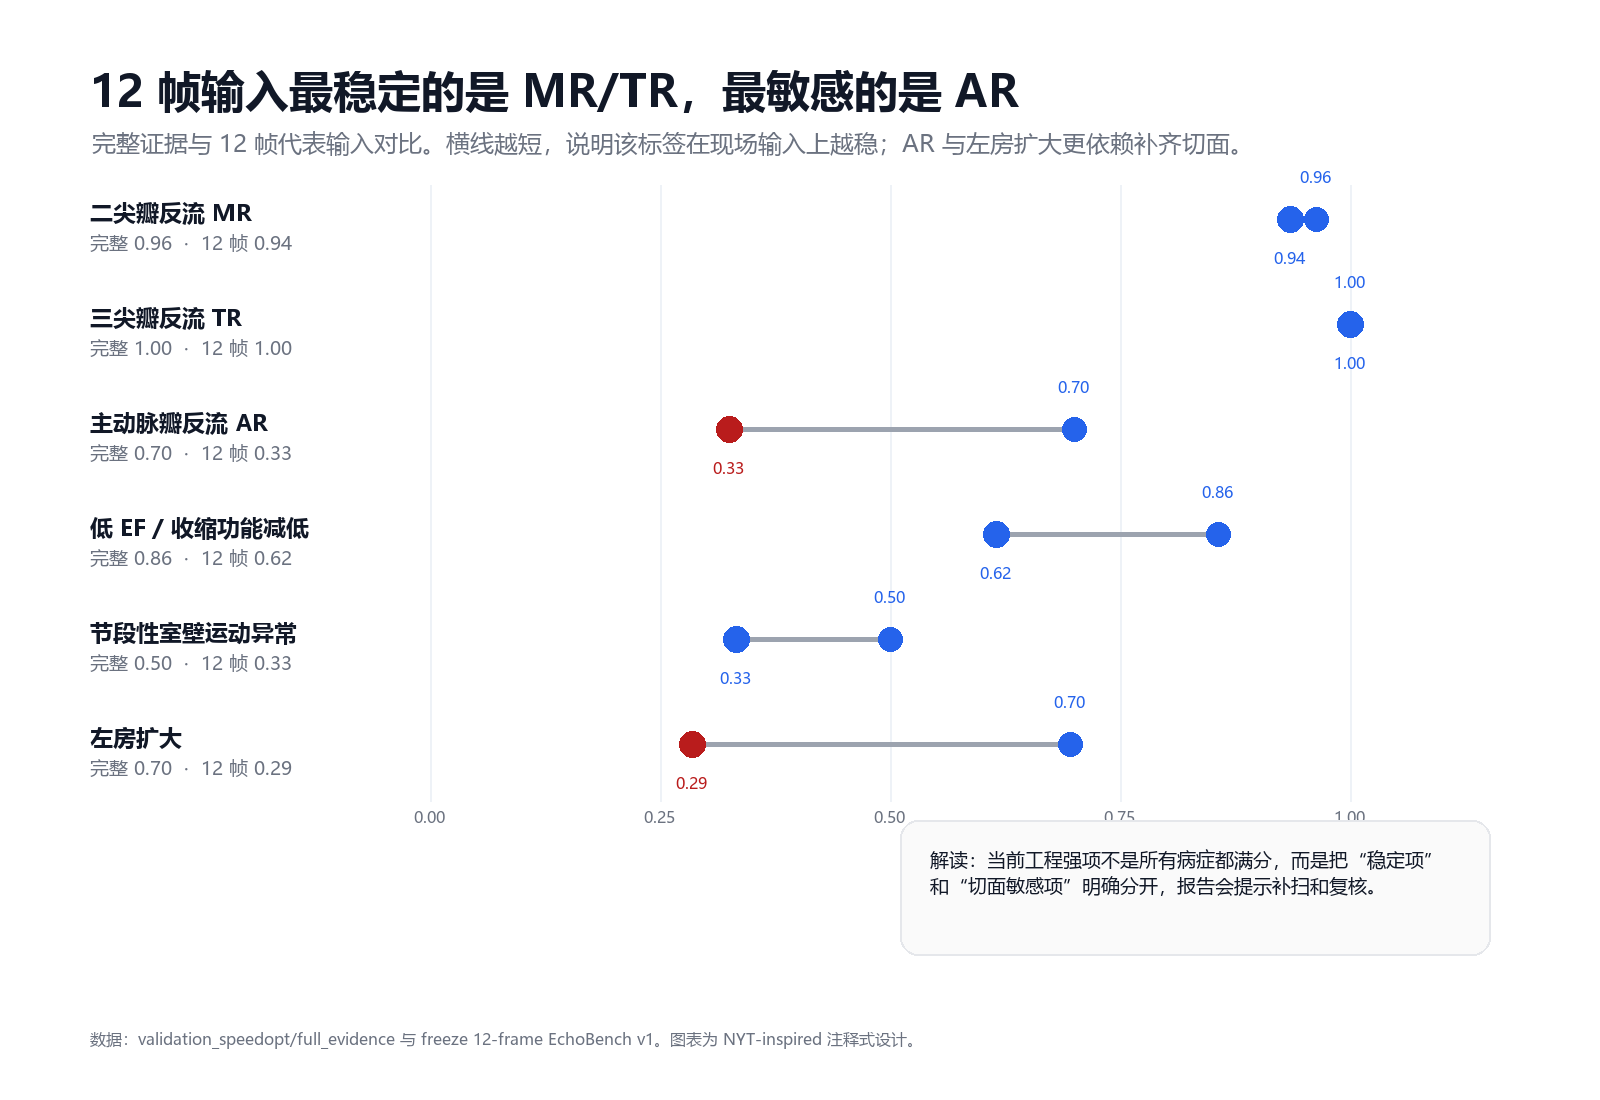
\includegraphics[width=\linewidth]{figures_nyt/nyt_fig1_f1_story.png}
  \caption{完整证据与 12 帧输入的 F1 对比。图表采用注释式新闻图表风格，强调稳定项和切面敏感项。}
\end{figure}

\begin{longtable}{p{4.2cm}rrrrrr}
\toprule
标签 & n & 阳性 & 准确率 & 敏感性 & 特异性 & F1\\
\midrule
\endfirsthead
\toprule
标签 & n & 阳性 & 准确率 & 敏感性 & 特异性 & F1\\
\midrule
\endhead
二尖瓣反流 MR & 60 & 55 & 0.933 & 0.964 & 0.600 & 0.964 \\
三尖瓣反流 TR & 60 & 60 & 1.000 & 1.000 & 0.000 & 1.000 \\
主动脉瓣反流 AR & 60 & 29 & 0.700 & 0.724 & 0.677 & 0.700 \\
低 EF / 收缩功能减低 & 60 & 6 & 0.967 & 1.000 & 0.963 & 0.857 \\
节段性室壁运动异常 & 60 & 3 & 0.967 & 0.333 & 1.000 & 0.500 \\
左房扩大 & 60 & 8 & 0.883 & 1.000 & 0.865 & 0.696 \\
\bottomrule
\caption{完整证据场景主要标签指标。}
\end{longtable}

\section{性能与成本}
旧 12 帧基线平均耗时 2.670 秒/例，当前 12 帧 warm-cache 平均耗时 0.711 秒/例，下降约 73.4\%。完整证据 warm-cache 平均 1.418 秒/例。本地 Gemma4 服务链路第 1 例诊断耗时约 69.2 秒，适合在演示中展示模型能力和结构化报告；规则链路适合快速证明输入输出合同和边缘特征链路。

\begin{figure}[htbp]
  \centering
  
\includegraphics[width=\linewidth]{figures_nyt/nyt_fig2_latency_story.png}
  \caption{规则链路、缓存和 Gemma4 服务链路的延迟对比。}
\end{figure}

\section{提交完整性}
当前提交材料集中在 PC 仓库，包括可运行代码、README、在线规则 demo、技术报告、数据来源说明、Apache-2.0 许可证、规则自检和多智能体审计。最后仍需人工完成的是 5 分钟内演示视频上传，并在提交表单中填写公开视频链接。

\begin{figure}[htbp]
  \centering
  
\includegraphics[width=\linewidth]{figures_nyt/nyt_fig3_submission_readiness.png}
  \caption{提交材料状态总览。}
\end{figure}

\section{取舍}
\begin{itemize}
  \item 为了离线和低成本，系统牺牲了云端大模型的算力弹性。
  \item 为了安全和可审计，最小病症由本地规则和校准层锁定，LLM 主要负责表达和解释。
  \item 为了兼容 DICOM/DCOM 和动图，代码保留了较复杂的输入解析、代表帧采样和相位推断。
  \item 为了现场复现稳定性，在线 demo 只做规则匹配；完整图像特征和 GGUF 推理以 PC V5 应用为准。
\end{itemize}

\section{局限与下一步}
当前 60 例为授权本地教学数据和报告链接标签，不是多中心外部临床验证，也不是多专家盲评共识。TR 在本批数据中几乎全阳性，特异性解释有限；AR、PR、严重反流、HCM、RWMA 等标签需要更多均衡样本。下一步应建立 2--3 位心超医生盲评表，计算 Cohen's Kappa、加权 Kappa 或 ICC，并补充外部数据验证。

\section{可复现命令}
\begin{verbatim}
python app.py --self-test-rule-only
python tools/submission_preflight.py
python submission/technical_report/make_nyt_style_figures.py
python submission/technical_report/build_latex_report.py --compile
\end{verbatim}

\begin{thebibliography}{9}
\bibitem{Leclerc2019} Leclerc, S., Smistad, E., Pedrosa, J., et al. (2019). Deep learning for segmentation using an open large-scale dataset in 2D echocardiography. \textit{IEEE Transactions on Medical Imaging}, 38(9), 2198--2210.
\bibitem{Ouyang2020} Ouyang, D., He, B., Ghorbani, A., et al. (2020). Video-based AI for beat-to-beat assessment of cardiac function. \textit{Nature}, 580(7802), 252--256.
\bibitem{Lang2015} Lang, R. M., Badano, L. P., Mor-Avi, V., et al. (2015). Recommendations for cardiac chamber quantification by echocardiography in adults. \textit{Journal of the American Society of Echocardiography}, 28(1), 1--39.e14.
\bibitem{Zoghbi2017} Zoghbi, W. A., Adams, D., Bonow, R. O., et al. (2017). Recommendations for noninvasive evaluation of native valvular regurgitation. \textit{Journal of the American Society of Echocardiography}, 30(4), 303--371.
\bibitem{Yu2002} Yu, Y., \& Acton, S. T. (2002). Speckle reducing anisotropic diffusion. \textit{IEEE Transactions on Image Processing}, 11(11), 1260--1270.
\end{thebibliography}

\end{document}
